\documentclass{beamer}
\usepackage{HECbeamer}
% \usepackage{pgfpages}
% \pgfpagesuselayout{4 on 1}[letterpaper, landscape, border shrink=5mm]
\title[\color{white}{MATH 60604A \S~6b - Clustered data example}]{\texorpdfstring{MATH 60604A \\Statistical modelling \\ \S~6b - Clustered data example}{MATH 60604A \\Statistical modelling \\ \S~6b - Clustered data example}}
\author{}
\institute{HEC Montréal\\
Department of Decision Sciences}
\date{} 

\begin{document}
\frame{\titlepage}

\begin{frame}[fragile]
\frametitle{Example: worker motivation}
We consider an example of clustered data.
\bi
\item  A large business collected data about its employees through a questionnaire. 
\item In this example, the response variable is \alert{worker motivation}. 
\item The level of worker motivation is defined as the \textbf{sum} of three items, namely
\bi

\item I share several of the company's values.
\item I feel loyal to the company.
\item I'm proud to tell people what company I work for.
\ei
measured on a Likert scale, ranging from strongly disagree ($1$) to strongly agree ($5$).
\item These data originates from

\begin{quote}
Lee, H.-J. and Peccei, R. (2007). \textsl{Organizational-Level Gender Dissimilarity and
Employee Commitment}. British Journal of Industrial Relations, \textbf{45}, 687--712.
\end{quote}
\ei
\end{frame}

\begin{frame}[fragile]
\frametitle{\texttt{motivation} data}
 The \code{motivation} data set contains the variables%, and the \SASlang{} code in \code{chapter7.sas}. 
\bi

\item \code{nunit}: number of employees in the unit (department).
\item \code{idunit}: id of unit in which the employee worked.
\item  \code{idemployee}: id of employee (within unit).
\item \code{yrserv}: years of service of employee.
\item \code{sex}: sex of employee, either male (\texttt{0}) or female (\texttt{1}).
\item  \code{agemanager}: age of the unit manager (in years).
\item \code{motiv}: worker motivation score.
\ei

\bi
\item  One possible source of correlation between observations is the \alert{unit (or department)} (group variable). 
\item It's possible that motivation is affected by what unit an employee belongs to due to factors such as temperature or type of work, among other things.
\ei
\end{frame}

\begin{frame}[fragile]
\frametitle{Summary statistics}
In the \texttt{motivation} data, units have different number of employees.
For example, unit $1$ has nine employees (three women and six men). 
\begin{center}
 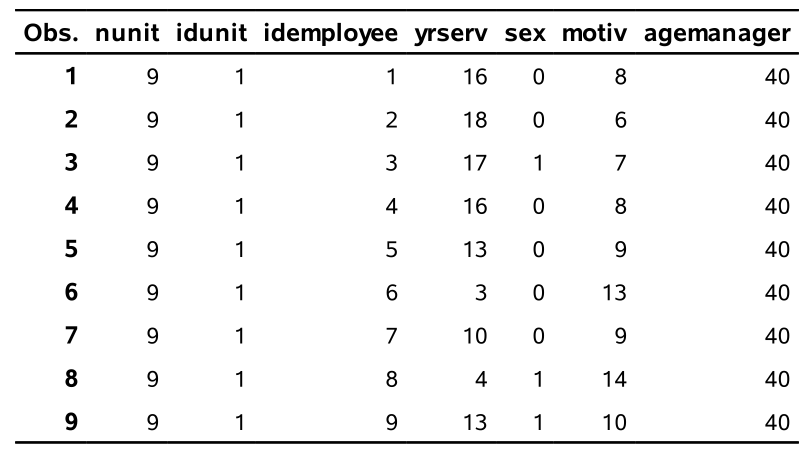
\includegraphics[width = 0.7\linewidth]{img/c6/slides7-e06}
\end{center}
{\small 
There are two types of variables, both of which can be included in the model: 
\be

\item those fixed for all individuals in the unit (\code{nunit} and \code{agemanager}) 
\item others that vary within unit (\code{yrserv} and \code{sex}). 
\ee
}
\end{frame}

\begin{frame}[fragile]
\frametitle{Grouping variable and study objective}
\bi
\item In the longitudinal \texttt{revenge} example, the group variable was the individual and we only had explanatory variables that were fixed for each person, i.e., fixed in time, with the exception of the time variable itself.
\item Here there are $100$ groups in total, and $1016$ observations in the file. 
\item The goal is to study the impact of sex, years of service, unit size, and of the age of the manager on worker mobilisation. 
\item However, we must account for the potential within-unit correlation. There is no natural ordering for the observations within a unit (contrary to the \texttt{revenge} example which contained repeated measurements over time).
\ei
\end{frame}


\begin{frame}[fragile]
\frametitle{Covariance structure for worker motivation}
\bi
\item We can consider the compound symmetry covariance structure to account for within-unit correlation. 
\bi

\item This means that we assume that the (conditional) correlation between a pair of observations in the same unit is always the same.
\ei
   
 \begin{tcolorbox}[colback=white, colframe=hecblue, title=\SASlang{} code for a linear model with equicorrelated errors]
 \begin{small}
\begin{verbatim}
proc mixed data=statmod.motivation method=reml; 
class idunit; 
model motiv = sex yrserv agemanager nunit / solution; 
repeated / subject=idunit type=cs r=1 rcorr=1; 
run;
\end{verbatim}
\end{small}
\end{tcolorbox}
\ei
\end{frame}
% 
%  \begin{frame}
% \frametitle{Model specifications}
% \begin{center}
% \includegraphics[scale=0.5]{Figures/long75.pdf}
% \includegraphics[scale=0.5]{Figures/long76.pdf}\\
% \includegraphics[scale=0.5]{Figures/long78.pdf}
% \includegraphics[scale=0.5]{Figures/long79.pdf}\\
% \includegraphics[scale=0.5]{Figures/long77.pdf}
% \end{center}
% \end{frame}

 \begin{frame}
\frametitle{Covariance matrix within-unit (unit 1)}
\begin{center}
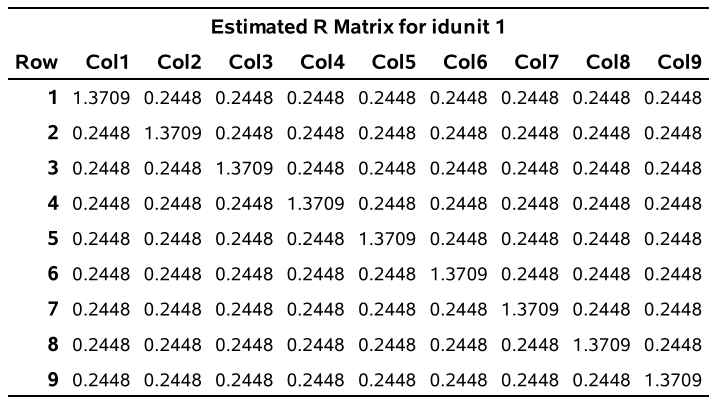
\includegraphics[width = 0.85\linewidth]{img/c6/slides7-e07}

\end{center}
\end{frame}

 \begin{frame}
\frametitle{Compound symmetry model}
\begin{center}
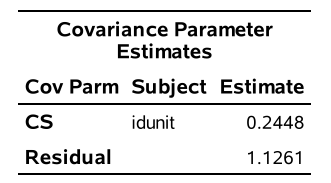
\includegraphics[width = 0.42\linewidth]{img/c6/slides7-e08}
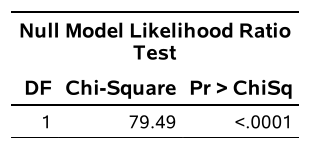
\includegraphics[width = 0.37\linewidth]{img/c6/slides7-e09}
\end{center}
\bi
\item The estimated covariance parameter from the compound symmetry model is $\hat{\tau} = 0.2448$. It is significantly different from $0$, suggesting a positive correlation between the worker motivation score between employees in the same unit, after adjusting for the effects of the explanatory variables. 
\item This estimated correlation between workers within-unit is $\hat{\rho} = 0.1785$. 
\ei
\end{frame}

% 
% \begin{frame}[fragile]
% \frametitle{Parameter coefficients as fixed effects}
% \bi
% \item  Consider the model we've used up to now:
% \begin{align*}
% Y_{ij}=\beta_0 + \beta_1 \mathrm{X}_{ij1}+\beta_2\mathrm{X}_{ij2}+\cdots+\beta_p\mathrm{X}_{ijp} + \varepsilon_{ij}
% \end{align*}
% for $i=1, \ldots, m$ and $j=1, \ldots, n_i$.
% \item In this model, $\bs{\beta}$ represent the \alert{fixed effects} which are the same for all individuals in the population. 
% \bi 
% \item The parameter $\beta_j$ describes how the mean of $Y$ varies as a function of $\mathrm{X}_j$ at the population level. 
% \ei
% 
% % \item The class of models for correlated data that we saw in the last section is a special case of a linear mixed model which we will outline soon.
% \ei
% \end{frame}

 \begin{frame}
\frametitle{Fixed effect estimates}
\begin{center}
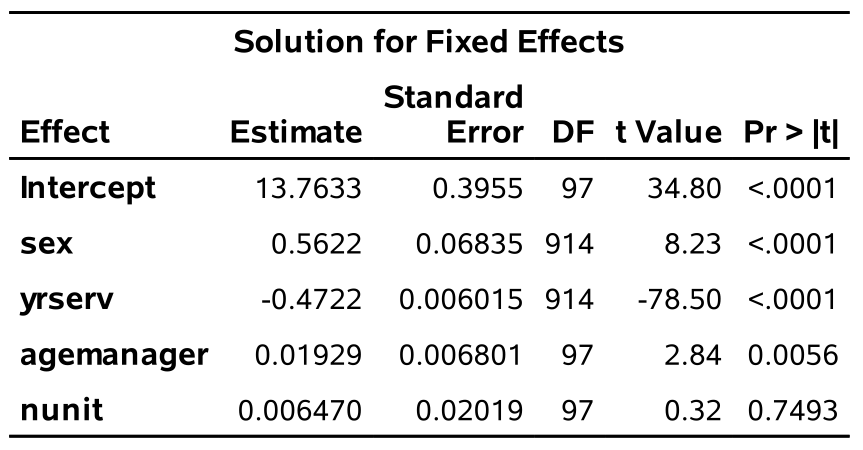
\includegraphics[width = 0.7\linewidth]{img/c6/slides7-e10}
\end{center}
\bi
\item The effects of three explanatory variables are significant: \code{sex}, \code{yrserv} and \code{agemanager}.
\bi

\item women are more motivated than men, on average. 
\item The longer a person has been employed at the company, the less (s)he is motivated. 
\item The older the manager, the more motivated the employee. 
\ei
\item However, the size of the unit is not significant.
\ei
\end{frame}


\begin{frame}[fragile]
\frametitle{Example: worker motivation}
\bi
\item It might be interesting to include an effect for the unit variable in the model. 
\item But, as we've already seen, when we include a fixed effect for each group, we lose the ability to estimate the effects of variables which are fixed within group. 
\item This would mean we could not include the variables \code{agemanager} or \code{nunit}.
\item However, there is still a way to include a ``group effect'' while also keeping the possibility of including variables which are fixed within group. 
\item We need to use \alert{random effects} instead of fixed effects, which can also be used to model the covariance structure.
\ei
\end{frame}
\end{document}
